\documentclass[a4paper,12pt]{article}
\usepackage[T2A]{fontenc}
\usepackage[utf8]{inputenc}
\usepackage[english]{babel}  % language changed to english
\usepackage{graphicx}
\usepackage{geometry}
\geometry{top=2cm,bottom=2cm,left=2.5cm,right=1.5cm}
\usepackage{float}
\usepackage{hyperref}
\usepackage{longtable}
\usepackage{caption}
\hypersetup{
    colorlinks=true,
    linkcolor=black,
    urlcolor=blue
}

\begin{document}

\begin{titlepage}
    \centering
    {\large \textbf{Electronic Chessboard}}\\[0.5cm]
    {\large \textbf{«ST-Mate»}}\\[2cm]
    {\Large \textbf{USER MANUAL}}\\[1cm]
    {\large \textbf{Version 1.0}}\\[3cm]
    \begin{figure}[H]
    \centering
    
\includegraphics[width=0.6\textwidth]{logo.png}
    \end{figure}
    \vfill
    \begin{flushright}
        \textit{Developed by: A.N. Kondratiev}\\
    \end{flushright}
    {\large \today}
\end{titlepage}

\tableofcontents

\newpage

% ========== 1 Introduction ==========
\section{Introduction}
\label{sec:introduction}

This document contains information necessary for the proper operation of the automated system «ST-Mate». 
The document describes the purpose and operating conditions, preparation for use, description of operations, user actions, as well as recommendations for troubleshooting and guidance on mastering the system.

\subsection{Scope of Application}
«ST-Mate» is designed as an intelligent chessboard for playing classical chess.
It is suitable for use in home environments, educational institutions, chess clubs and other places.

\subsection{Brief Description of Automation Capabilities}
«ST-Mate» provides the following functions:
\begin{itemize}
    \item Automatic detection of piece positions on the board.
    \item Highlighting of legal moves for each piece.
    \item Move suggestions at the press of a button.
    \item Game management in three modes.
    \item Bluetooth wireless interface for remote monitoring and control.
\end{itemize}

\subsection{List of Operational Documentation}
Operational documentation includes:
User Manual (this document) - contains information for users about the purpose, operating conditions, preparation for use, description of operations, and troubleshooting recommendations.

% ========== 2 Purpose and Operating Conditions ==========
\section{Purpose and Operating Conditions}
\label{sec:purpose}

\subsection{Purpose of ST-Mate}
«ST-Mate» is an intelligent chessboard designed for playing classical chess in three modes:
\begin{itemize}
    \item Player controlling white pieces against the built-in chess engine;
    \item Two-player mode without engine intervention.
    \item Player controlling black pieces against the built-in chess engine;
\end{itemize}

«ST-Mate» automatically recognises piece positions, highlights legal moves, provides hints, and manages the game.

\subsection{Technical Specifications}

\begin{itemize}
    \item Overall dimensions (L×W×H): 455×455×45 mm.
    \item Playing field size: 400×400 mm.
    \item Square size: 50×50 mm.
    \item Power connector: USB Type-C.
    \item Supply voltage: 5 V.
    \item Maximum current consumption: 500 mA.
    \item Microcontroller: STM32F103C8T6.
    \item Piece position sensors: 64 Hall effect sensors SS49E.
    \item Square illumination: addressable LED strip WS2813.
    \item Chess engine: micro-Max version 4.8 by H.G. Muller.
    \item Wireless interface: Bluetooth, device name «ST-Mate».
\end{itemize}

\subsection{Operating Conditions}
The «ST-Mate» chessboard is intended for operation at temperatures from +5 to +30 °C and relative humidity not exceeding 80 \% without condensation.
Exposure to direct sunlight, vibration, shocks, or liquids is not allowed.

% ========== 3 Preparation for Use ==========
\section{Preparation for Use}
\label{sec:preparation}

\subsection{Unpacking and Inspection}
Remove the «ST-Mate» chessboard from its packaging.
Ensure there is no visible mechanical damage to the housing, board, or pieces.
Check the contents.

The package includes:
\begin{itemize}
    \item Electronic chessboard - 1 pc.
    \item Pieces with magnets (32 pcs.) - 1 set.
    \item User manual - 1 pc.
\end{itemize}

\subsection{Connecting to a Power Source}
Make sure the power supply (not included) meets the requirements (USB power adapter 5 V / at least 500 mA or a USB port of a computer).
The USB Type-C cable (not included) must be undamaged, and the connectors must be free of dirt or deformation.\\
For first-time use, perform the following steps with no pieces on the board:
\begin{enumerate}
    \item Connect one end of the cable to the power source.
    \item Connect the other end (USB Type-C) to the connector on the rear panel of the ST-Mate.
    \item After power is applied, the «ST-Mate» chessboard performs a self-test and calibration: all LEDs briefly light up, then the board enters the waiting state for the initial setup of pieces.
\end{enumerate}

\subsection{Functionality Check}
After connecting the power and completing the self-test, verify the following:
\begin{enumerate}
    \item Orient the board so that the nearest corner square on the right side of each player is white.
    \item The first two ranks (ranks 1 and 2) from the white side and the two ranks (ranks 7 and 8) from the black side should flash red.
    \item Squares on which pieces are placed are illuminated in green.
    \item Ranks 3–6 are not lit if they have no pieces; otherwise they flash red. See section \ref{sec:initial-position} \nameref{sec:initial-position}.
    \item If white and black pieces are placed on the wrong sides (sides swapped), they flash red. See section \ref{sec:initial-position} \nameref{sec:initial-position}.
\end{enumerate}
If any of the above conditions are not met, perform a reset using the «RESET» button and repeat the verification procedure.
If the problem persists, refer to section \ref{sec:troubleshooting} \nameref{sec:troubleshooting}.


% ========== 4 Description of Operations ==========
\section{Description of Operations}
\label{sec:operations}

\subsection{Controls}
On the front panel (from left to right):
\begin{enumerate}
    \item Logo.
    \item \textbf{«HINT»} button - when pressed, shows a suggested move for the side whose turn it is.
    \item Switch - has three positions corresponding to the game modes.
    \item \textbf{«RNG»} button (random number generator) - activates the mode in which the engine makes random moves (useful for training).
\end{enumerate}
On the rear side of the board (from left to right):
\begin{enumerate}
    \item \textbf{RESET} button - forces a microcontroller reboot.
    \item \textbf{USB} power connector.
\end{enumerate}

\subsection{Selecting the Game Mode}
The switch is located on the front panel of the «ST-Mate» chessboard.

Game modes:
\begin{itemize}
    \item \textbf{WvE} - the player controls the white pieces; the controller moves black.
    \item \textbf{PvP} - both players move alternately; the controller only tracks piece positions and provides hints.
    \item \textbf{BvE} - the player controls the black pieces; the controller moves white.
\end{itemize}
When the mode is changed using the switch, the game is automatically reset. To start a new game, the pieces must be placed in the initial position (see section \ref{sec:initial-position} \nameref{sec:initial-position}).

After setting up the pieces and selecting the mode, the «ST-Mate» chessboard is ready for play.

\subsection{Initial Position of Pieces}
\label{sec:initial-position}
Before starting a game, place the pieces in the initial position corresponding to the standard starting position (Fig. \ref{fig:startpos}).
The pieces are recognised automatically by the built-in Hall effect sensors.

\begin{figure}[H]
    \centering
    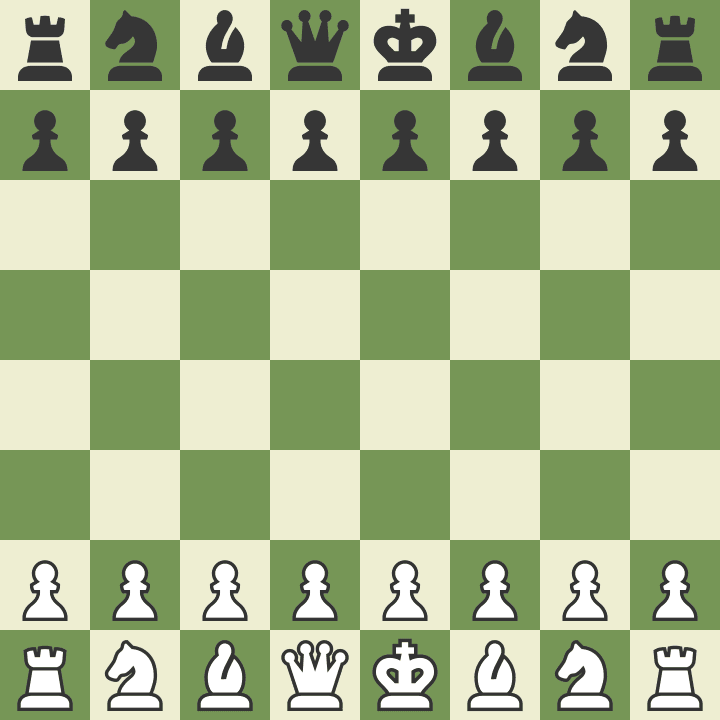
\includegraphics[width=0.5\textwidth]{chess position.png}
    \caption{Initial position of pieces on the board}
    \label{fig:startpos}
\end{figure}

\textbf{Important:} After each mode change or when power is applied, the board automatically enters the waiting state for the initial setup.
The pieces must be manually placed in their correct squares. Once the setup is complete, the controller automatically detects all pieces and is ready for play.


\subsection{Performing a Move}
According to chess rules, players alternate moves. White moves first.
The move procedure includes the following steps:
\begin{enumerate}
    \item The player whose turn it is picks up a piece of their colour and places it on the destination square. The Hall effect sensors detect the change in piece positions.
    \item If the move is legal according to chess rules, the controller confirms it by highlighting the squares. The move is considered made, and the turn passes to the opponent (or the controller).
    \item If an illegal move is attempted (e.g., moving to a square not reachable by the piece, or moving into check), the squares flash red and the move is not accepted. The player must return the piece to its original square and choose another move.
\end{enumerate}

Capturing a piece involves the following steps:
\begin{enumerate}
    \item The player whose turn it is picks up a piece of their colour.
    \item The player also picks up the opponent’s piece.
    \item The player places their own piece on the square previously occupied by the opponent’s piece.
\end{enumerate}
If the capture is legal, the controller confirms the move by highlighting the squares involved.

\subsection{Special Moves}
\textbf{Castling:} A special move consisting of moving the king two squares horizontally toward a rook of the same colour, and then moving the rook to the square adjacent to the king on the opposite side.
Each side may castle once during the game.

Castling kingside is shown in Fig. \ref{fig:kingside castling}.
\begin{figure}[H]
    \centering
    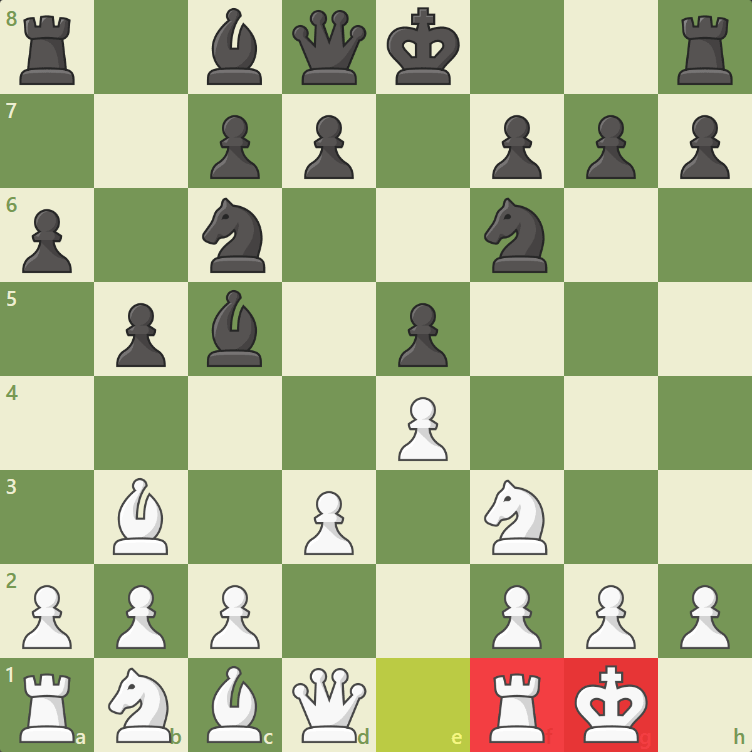
\includegraphics[width=0.4\textwidth]{kingside castling.png}
    \caption{Castling kingside}
    \label{fig:kingside castling}
\end{figure}

Castling queenside is shown in Fig. \ref{fig:queenside castling}.
\begin{figure}[H]
    \centering
    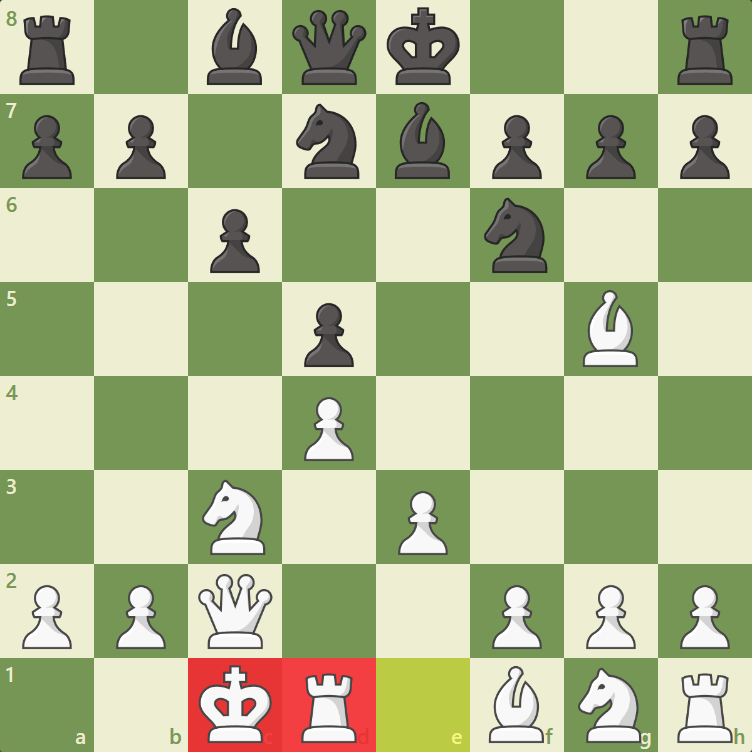
\includegraphics[width=0.4\textwidth]{queenside castling.png}
    \caption{Castling queenside}
    \label{fig:queenside castling}

\end{figure}

The castling procedure includes the following steps:
\begin{enumerate}
    \item The player whose turn it is picks up their king and places it on the destination square.
    \item Then they move their rook to the square adjacent to the king on the opposite side.
    \item The castling procedure will indicate the positions of the king and rook.
    \item If the move is legal, the controller confirms it by highlighting the squares. The turn passes to the opponent (or the controller).
    \item If an illegal move is attempted (e.g., moving through check or into check), the squares flash red and the move is not accepted. The player must return the pieces to their original squares and choose another move.
\end{enumerate}

\textbf{En passant capture:} A special pawn capture where a pawn captures an opponent’s pawn that has just advanced two squares from its starting square. The capturing pawn moves to the square that the opponent’s pawn passed over, as if the opponent’s pawn had advanced only one square. The capture is only possible on the move immediately following the opponent’s pawn advance.

The en passant capture is shown in Fig. \ref{fig:en passant}.
\begin{figure}[H]
    \centering
    \includegraphics[width=0.4\textwidth]{en passant.png}
    \caption{En passant capture}
    \label{fig:en passant}
\end{figure}

The en passant procedure includes the following steps:
\begin{enumerate}
    \item The player whose turn it is picks up their pawn.
    \item They then pick up the opponent’s pawn and remove it from the board.
    \item They place their own pawn on the square that was passed over by the opponent’s pawn.
    \item If the move is legal, the controller confirms it by highlighting the squares. The turn passes to the opponent (or the controller).
    \item If an illegal move is attempted, the squares flash red and the move is not accepted. The player must return the piece to its original square and choose another move.
\end{enumerate}

\textbf{Promotion:} A special move in which a pawn that reaches the last rank is promoted to another piece.
In the current software version, the pawn automatically promotes to a queen. The option to choose a piece will be added in future updates.

The promotion procedure includes the following steps:
\begin{enumerate}
    \item The player whose turn it is picks up their pawn on the second last rank.
    \item They replace it with a queen of the same colour and place it on the destination square.
    \item If a capture is available on the last rank, the player makes the capture and places the queen on that square.
    \item If the move is legal, the controller confirms it by highlighting the squares. The turn passes to the opponent (or the controller).
    \item If an illegal move is attempted, the squares flash red and the move is not accepted. The player must return the piece to its original square and choose another move.
\end{enumerate}

\subsection{Using the HINT Button}
The «HINT» button is located on the side panel of the «ST-Mate» chessboard.
The hint does not affect the turn order and does not automatically make a move.

\subsection{Using the RNG Button}
The «PRNG» button is located on the side panel of the «ST-Mate» chessboard.
The RNG button is intended to enable random move generation by the controller in modes involving the chess engine.
The RNG mode can only be activated when the board is powered on or reset.

\subsection{Reset and Restart}
If a forced reset of the «ST-Mate» chessboard is required (e.g., in case of a freeze or to start a new game), use the «RESET» button located next to the USB Type-C connector.
A short press of the button reboots the microcontroller and repeats the initialisation procedure.
After a reset, the pieces must be placed in the initial position again.

\subsection{Bluetooth Control}
For remote control and monitoring, the board is equipped with a Bluetooth interface.
Connect to it using a smartphone, tablet, or computer with any terminal client (e.g., \textit{Serial Bluetooth Terminal}).
After connection, a text-based command protocol is available.
Commands are transmitted in UTF-8 encoding and end with the characters \texttt{\textbackslash{r}\textbackslash{n}} (carriage return and line feed).

\subsection{Connection}
When the «ST-Mate» chessboard is powered on, it becomes available for Bluetooth connection under the name \texttt{ST-Mate}.

% ========== Troubleshooting ==========
\section{Troubleshooting}
\label{sec:troubleshooting}

Table \ref{tab:errors} lists possible abnormal situations and recommended actions.
\begin{table}[H]
    \centering
    \begin{tabular}{|p{0.3\textwidth}|p{0.6\textwidth}|}
        \hline
        \textbf{Situation} & \textbf{User Action} \\
        \hline
        The «ST-Mate» chessboard does not turn on, no backlight & 
        Check the USB Type-C cable connection, ensure the power supply provides 5 V and at least 500 mA.
        Try a different cable or USB port. \\
        \hline
        Pieces are not recognised (no reaction to movement) & 
        Ensure the pieces are from the original set and placed exactly in the centre of squares.
        If necessary, press «RESET» and set up the pieces again. \\
        \hline
        Erratic backlight (random flashing) & 
        Possible influence of external magnetic fields.
        Remove sources of strong magnetic fields.
        Perform a reset. \\
        \hline
        Piece highlighting does not match their positions &
        Increase the sensor trigger level in settings by 5–10 units.
        Increase the smoothing coefficient in settings by 1–2 units.
        Check the power supply for compliance with requirements.
        Reduce backlight brightness in settings. \\
        \hline
        After calibration, sensors do not react to pieces & 
        Make sure calibration was performed with no pieces on the board.
        Repeat forced calibration.
        Adjust the trigger level and smoothing coefficient. \\
        \hline
        The engine does not make a move in modes with controller & 
        Verify the correct mode is selected and that it is the controller’s turn.
        If the delay exceeds 10 seconds, press «HINT» to initiate a move. \\
        \hline
        Bluetooth does not work, ST-Mate not in device list &
        Ensure ST-Mate is powered on. Contact the ST-Mate developer. \\
        \hline
    \end{tabular}
    \caption{Abnormal situations and remedies}
    \label{tab:errors}
\end{table}

% ========== Guidance for Mastering ==========
\section{Guidance for Mastering}
\label{sec:usage}
To quickly become familiar with the «ST-Mate» chessboard, it is recommended to:
\begin{itemize}
    \item Carefully read this manual, especially sections \ref{sec:operations} \nameref{sec:operations} and \ref{sec:troubleshooting} \nameref{sec:troubleshooting}.
    \item Familiarise yourself with the FIDE laws of chess. Link to the official FIDE handbook: \url{https://handbook.fide.com/} (accessed: 01.04.2026).
    \item Start with «Player vs Player» mode without using hints, to get used to the physical interaction with the board and understand how moves are recognised.
    \item After mastering basic operations, move on to playing against the controller, using hints to study tactical techniques.
    \item If in doubt about the correctness of the piece positions, use the «Reset» button and start a new game.
\end{itemize}

\subsection{Visual User Messages}

The «ST-Mate» chessboard uses various methods to inform the user about the current state and events.
It is advisable to use the standard colour theme (THEME:0) for mastering, which intuitively displays legal moves and errors.
The following examples of light indication are given for the standard theme.

For the initial setup and waiting for the game to start, squares of ranks 1 and 2 from the white side and ranks 7 and 8 from the black side are lit in red, while the four central ranks are not lit.
As soon as the pieces are placed in their correct squares, the board recognises them and turns off the backlight.
When a piece is selected, the square it occupies starts flashing white. Legal moves for the selected piece are illuminated in white.
Once the piece is moved to a new square, the completed move is highlighted in yellow, and the turn passes to the opponent (or the controller).
If an illegal move is attempted, the squares flash red.
When the «HINT» button is pressed to show a recommended move, the squares involved in the suggestion are lit in blue.
During castling, the squares where the king moves are lit white. After the king moves, the completed move is highlighted yellow.
Then the rook move is indicated with white light; after the rook is moved, the turn passes to the opponent (or the controller).
When delivering a check, the attacking piece flashes blue, while the king in check flashes red.
When checkmate occurs, the attacking piece flashes green, and the mated king flashes red. The game ends.
In a stalemate situation, the kings flash yellow. The game ends.
After the game ends, any movement of a piece resets the board to waiting for the initial setup for a new game, and ranks 1–2 from white and 7–8 from black light up red again.

\subsection{Text User Messages via Bluetooth}
Using Bluetooth to obtain detailed information about moves and game state can be useful for analysis and learning, but is not required for basic operation.
Via Bluetooth, ST-Mate can send text messages informing the user about the current state, move results, and other events.
Completed moves are output in algebraic notation (e.g., “e2e4” for a pawn move from e2 to e4).
Moves that were rejected due to rule violations are accompanied by an error message (e.g., “White make invalid move e2e5”).
At the end of the game, the result is displayed (e.g., “1-0” for white win, “0-1” for black win, “1/2-1/2” for draw).
The PGN of the current game is also output, allowing it to be saved and analysed. Output for initialisation, start, game progress, and result in PGN format is shown in Fig. \ref{fig:log}.

\begin{figure}[H]
    \centering
    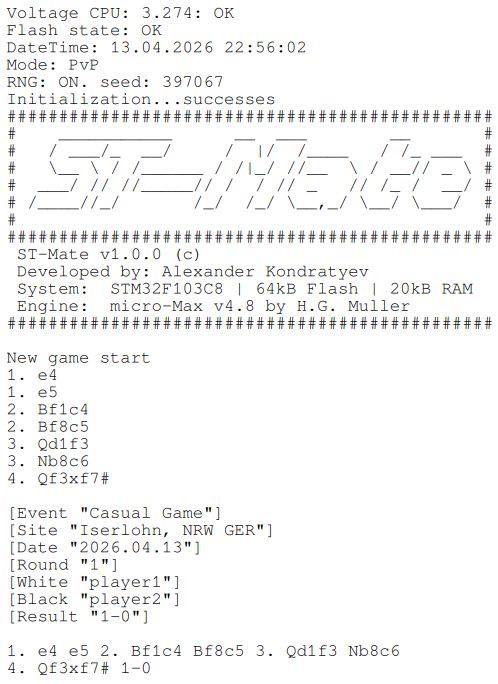
\includegraphics[width=0.6\textwidth]{log.png}
    \caption{Bluetooth message log}
    \label{fig:log}
\end{figure}

\subsection{Sending Commands}
After connecting to the board via Bluetooth, the user can send text commands.
Commands are case-insensitive.
Supported queries and commands are listed in Appendix A.

\subsection{Usage Examples}
\begin{verbatim}
> BRIGHT:80\r\n 
Brightness set:80\r\n
> THEME:5\r\n
Theme set:5\r\n
> TRIGLV?\r\n
Trigger level:40\r\n
\end{verbatim}

% ========== Technical Maintenance ==========
\section{Technical Maintenance}
\label{sec:maintenance}

To avoid injury and damage, as well as to ensure a long service life of the «ST-Mate» chessboard, the following maintenance recommendations should be observed.
\begin{itemize}
    \item Do not disassemble the device yourself, as this may cause injury or damage.
    \item Keep the board and pieces clean; avoid liquid ingress into the housing.
    \item Regularly check the integrity of the power cable and the USB Type-C connector. Do not use damaged cables.
    \item For storage and transportation, use the original packaging or equivalent protection against shocks and vibrations.
    \item Do not expose the device to extreme temperatures, direct sunlight, or strong magnetic fields.
\end{itemize}
If malfunctions occur, refer to the “Troubleshooting” section or contact the developers.

\subsection{Sensor Calibration}
Calibration is recommended upon first use, after replacing the power supply or cable, or when operating conditions (temperature, humidity) change.
The calibration table is stored in non-volatile memory.
Calibration is performed automatically at power-on or reset if there are no pieces on the board.\\
There are two ways to perform forced calibration:

\begin{enumerate}
    \item With the «HINT» button held down when applying power or pressing the «RESET» button.
    \item Via the terminal command \texttt{CALIBRATE\textbackslash{r}\textbackslash{n}} over Bluetooth.
\end{enumerate}

To perform forced calibration:
\begin{itemize}
    \item Remove all pieces from the board.
    \item Use one of the methods to start calibration.
    \item Wait for the process to finish (about 5 seconds).
\end{itemize}

\subsection{Storage and Transportation}
Store the «ST-Mate» chessboard in a dry, clean place at a temperature between +5 and +30 °C.
For transportation, use the original packaging or equivalent protection against shocks and vibrations.
Avoid exposure to direct sunlight, moisture, extreme temperatures, and mechanical damage.

\subsection{Surface Care}
Wipe the housing and pieces with a soft, slightly damp cloth. Do not allow liquid to enter the housing. Do not use abrasive cleaning agents.


\newpage
% ========== List of Abbreviations ==========
\section{List of Abbreviations}
\label{sec:abbreviations}

\begin{itemize}
    \item AS - automated system.
    \item USB - Universal Serial Bus.
    \item LED - Light Emitting Diode.
    \item Bluetooth - wireless technology for short-range data exchange.
    \item PGN - Portable Game Notation, a format for recording chess games.
    \item FEN - Forsyth-Edwards Notation, a format for describing a chess position.
    \item RNG - Random Number Generator.
    \item STM32 - family of 32-bit microcontrollers from STMicroelectronics.
    \item SS49E - Hall effect sensor used to detect the presence of a magnetic field.
    \item WS2813 - type of addressable LED strip.
    \item micro-Max - compact chess engine developed by H.G. Muller. Source code available at: \url{https://home.hccnet.nl/h.g.muller/umax4_8.c} (accessed: 01.04.2026).
\end{itemize}

\newpage

% ========== Developer Information and Contact Details ==========
\section{Developer Information and Contact Details}
\label{sec:developers}

\begin{itemize}
    \item \textbf{Developer of the ST-Mate chessboard:} Kondratiev Alexander Nikolaevich.\\
          Email: \texttt{alexander.kondratyev.dev@gmail.com}\\
          Telegram: \url{https://t.me/kondratyev_an}
    \item \textbf{Developer of the micro-Max chess engine:} H.G. Muller.\\
          Homepage: \url{https://home.hccnet.nl/h.g.muller/} (accessed: 01.04.2026).
\end{itemize}
All questions regarding operation, configuration, and modification of the «ST-Mate» chessboard should be directed to the developers.

\newpage

% ========== APPENDICES ==========
\clearpage
\section*{Appendix A. Command Protocol}
\addcontentsline{toc}{section}{Appendix A. Command Protocol}
\label{sec:protocol}

\begin{longtable}{|p{0.15\textwidth}|p{0.80\textwidth}|}
\hline
\textbf{Command} & \textbf{Description} \\ \hline
\endfirsthead
\hline
\textbf{Command} & \textbf{Description} \\ \hline
\endhead
\hline
\endfoot
\multicolumn{2}{|c|}{\textbf{Service Commands}} \\ \hline
\texttt{REBOOT} & Reboot the device (analogous to pressing the «RESET» button). \\ \hline
\texttt{SERVICE:X} & Enable/disable service mode. X=0 - disabled, X=1 - enabled. \\ \hline
\texttt{VOLT?} & Request processor supply voltage (returns value in millivolts). \\ \hline
\texttt{CALIBRATE} & Start sensor calibration (board must be empty). \\ \hline
\texttt{TRIGLV?} & Request current trigger level of sensors (default 25). \\ \hline
\texttt{TRIGLV:X} & Set sensor trigger level (X is an integer depending on calibration). \\ \hline
\texttt{ALPHA?} & Request current exponential smoothing coefficient (default 8). \\ \hline
\texttt{ALPHA:X} & Set exponential smoothing coefficient (X is an integer). \\ \hline
\multicolumn{2}{|c|}{\textbf{User Commands}} \\ \hline
\texttt{EVENT?} & Request tournament or match name. \\ \hline
\texttt{EVENT:X} & Set tournament or match name (e.g., EVENT:Casual Game). \\ \hline
\texttt{SITE?} & Request venue. \\ \hline
\texttt{SITE:X} & Set venue (e.g., SITE:Moscow). \\ \hline
\texttt{TIME?} & Request current time. \\ \hline
\texttt{TIME:X} & Set current time (X is a string in the format dd.mm.yy HH:MM:SS). \\ \hline
\texttt{ROUND?} & Request round number. \\ \hline
\texttt{ROUND:X} & Set round number (e.g., ROUND:1). \\ \hline
\texttt{WHITE?} & Request name of the player playing white. \\ \hline
\texttt{WHITE:X} & Set name of the player playing white (e.g., WHITE:Alice). \\ \hline
\texttt{BLACK?} & Request name of the player playing black. \\ \hline
\texttt{BLACK:X} & Set name of the player playing black (e.g., BLACK:Bob). \\ \hline
\texttt{FEN?} & Request current position in FEN format. \\ \hline
\texttt{PGN?} & Request current game in PGN format. \\ \hline
\texttt{SEED?} & Request current seed for the random number generator. \\ \hline
\texttt{SEED:X} & Set seed for the random number generator (X is an integer or string). \\ \hline
\texttt{BRIGHT?} & Request current backlight brightness level. \\ \hline
\texttt{BRIGHT:X} & Set backlight brightness (0–100). Example:\texttt{BRIGHT:50}. \\ \hline
\texttt{THEME:X} & Set colour theme (0–11). List of themes is given in \nameref{sec:themes}. \\ \hline
\texttt{HINTBTN:X} & Enable/disable the HINT button. X=0 - button inactive, X=1 - active. \\ \hline
\end{longtable}

\clearpage
\section*{Appendix B. Colour Schemes for Backlight}
\addcontentsline{toc}{section}{Appendix B. Colour Schemes for Backlight}
\label{sec:themes}

\begin{center}
\begin{tabular}{|c|l|}
\hline
\textbf{Code} & \textbf{Theme Name} \\ \hline
    0 & Default - standard theme (default) \\
    1 & Neon Night - bright neon colours \\
    2 & Forest Glade - natural green and brown shades \\
    3 & Ocean Breeze - marine theme with blue tones \\
    4 & Royal Purple - noble purple shades \\
    5 & Autumn Sunset - warm autumn colours \\
    6 & Arctic Ice - cool pastel tones \\
    7 & Desert Sand - sandy and earthy shades \\
    8 & Candy Land - bright candy colours \\
    9 & Midnight Oil - dark saturated tones \\
    10 & Spring Meadow - fresh spring colours \\
    11 & Classic Elegance - restrained classic palette \\
\hline
\end{tabular}
\end{center}

\end{document}